% \documentclass{beamer}
\documentclass[handout]{beamer}
\usetheme{Boadilla}

\usepackage[document]{ragged2e}
\usepackage[utf8]{inputenc}
\usepackage[absolute,overlay]{textpos}
\TPGrid[10 mm,8 mm]{9}{8}

\setbeamertemplate{navigation symbols}{}
\setbeamertemplate{footline}[frame number]{}
\definecolor{Yellow}{rgb}{1.0, 1.0, 0.0}
\definecolor{Black}{rgb}{0.0, 0.0, 0.0}
\setbeamercolor{title}{fg=Yellow}
\setbeamertemplate{itemize subitem}{\color{orange}$\blacktriangleright$}
\defbeamertemplate*{title page}{customized}[1][]
{
	\centering
	\usebeamercolor[fg]{title}
	\usebeamerfont{title}\inserttitle\par
	\usebeamerfont{subtitle}\usebeamercolor[fg]{subtitle}\insertsubtitle\par
	\bigskip \bigskip \bigskip \bigskip \bigskip
	\usebeamercolor[Black]{author}
	\usebeamerfont{author}\insertauthor\par
	\bigskip \bigskip
	\usebeamerfont{date}\insertdate\par
}

\makeatletter
\setbeamertemplate{frametitle}{
    \ifbeamercolorempty[bg]{frametitle}{}{\nointerlineskip}
    \@tempdima=\textwidth
    \advance\@tempdima by\beamer@leftmargin
    \advance\@tempdima by\beamer@rightmargin
    \hspace*{1cm}
    \begin{beamercolorbox}[sep=0.3cm,center,wd=\the\@tempdima]{frametitle}
				\usebeamercolor[Yellow]{}
        \usebeamerfont{frametitle}
        \vbox{}\vskip-1ex
        \vbox{}\vskip-1ex
        \if@tempswa\else\csname beamer@ftecenter\endcsname\fi%
        \strut\insertframetitle\strut\par
        {
            \ifx\insertframesubtitle\@empty
            \else
            {\usebeamerfont{framesubtitle}\usebeamercolor[fg]{framesubtitle}\insertframesubtitle\strut\par}
            \fi
        }
        \vskip-1ex
        \if@tempswa\else\vskip-.3cm\fi
    \end{beamercolorbox}
}
\makeatother

\newcommand{\parx}{
	\setlength{\parindent}{4em}
	\par}

\newcommand{\ui}[1]{
	\begin{frame}
		\frametitle{User-Interface Mockup and Design}
		\begin{figure}
			\includegraphics[height=0.6\textheight,keepaspectratio]{UI/#1.png}
		\end{figure}
	\end{frame}
}

\title{CodeNect: Visual Programming Software for Learning Fundamentals of Programming}
\author{Brandon B. Lim-it, Jaykel O. Punay}
\date{May, 2021}

\begin{document}

\setbeamertemplate{background}
{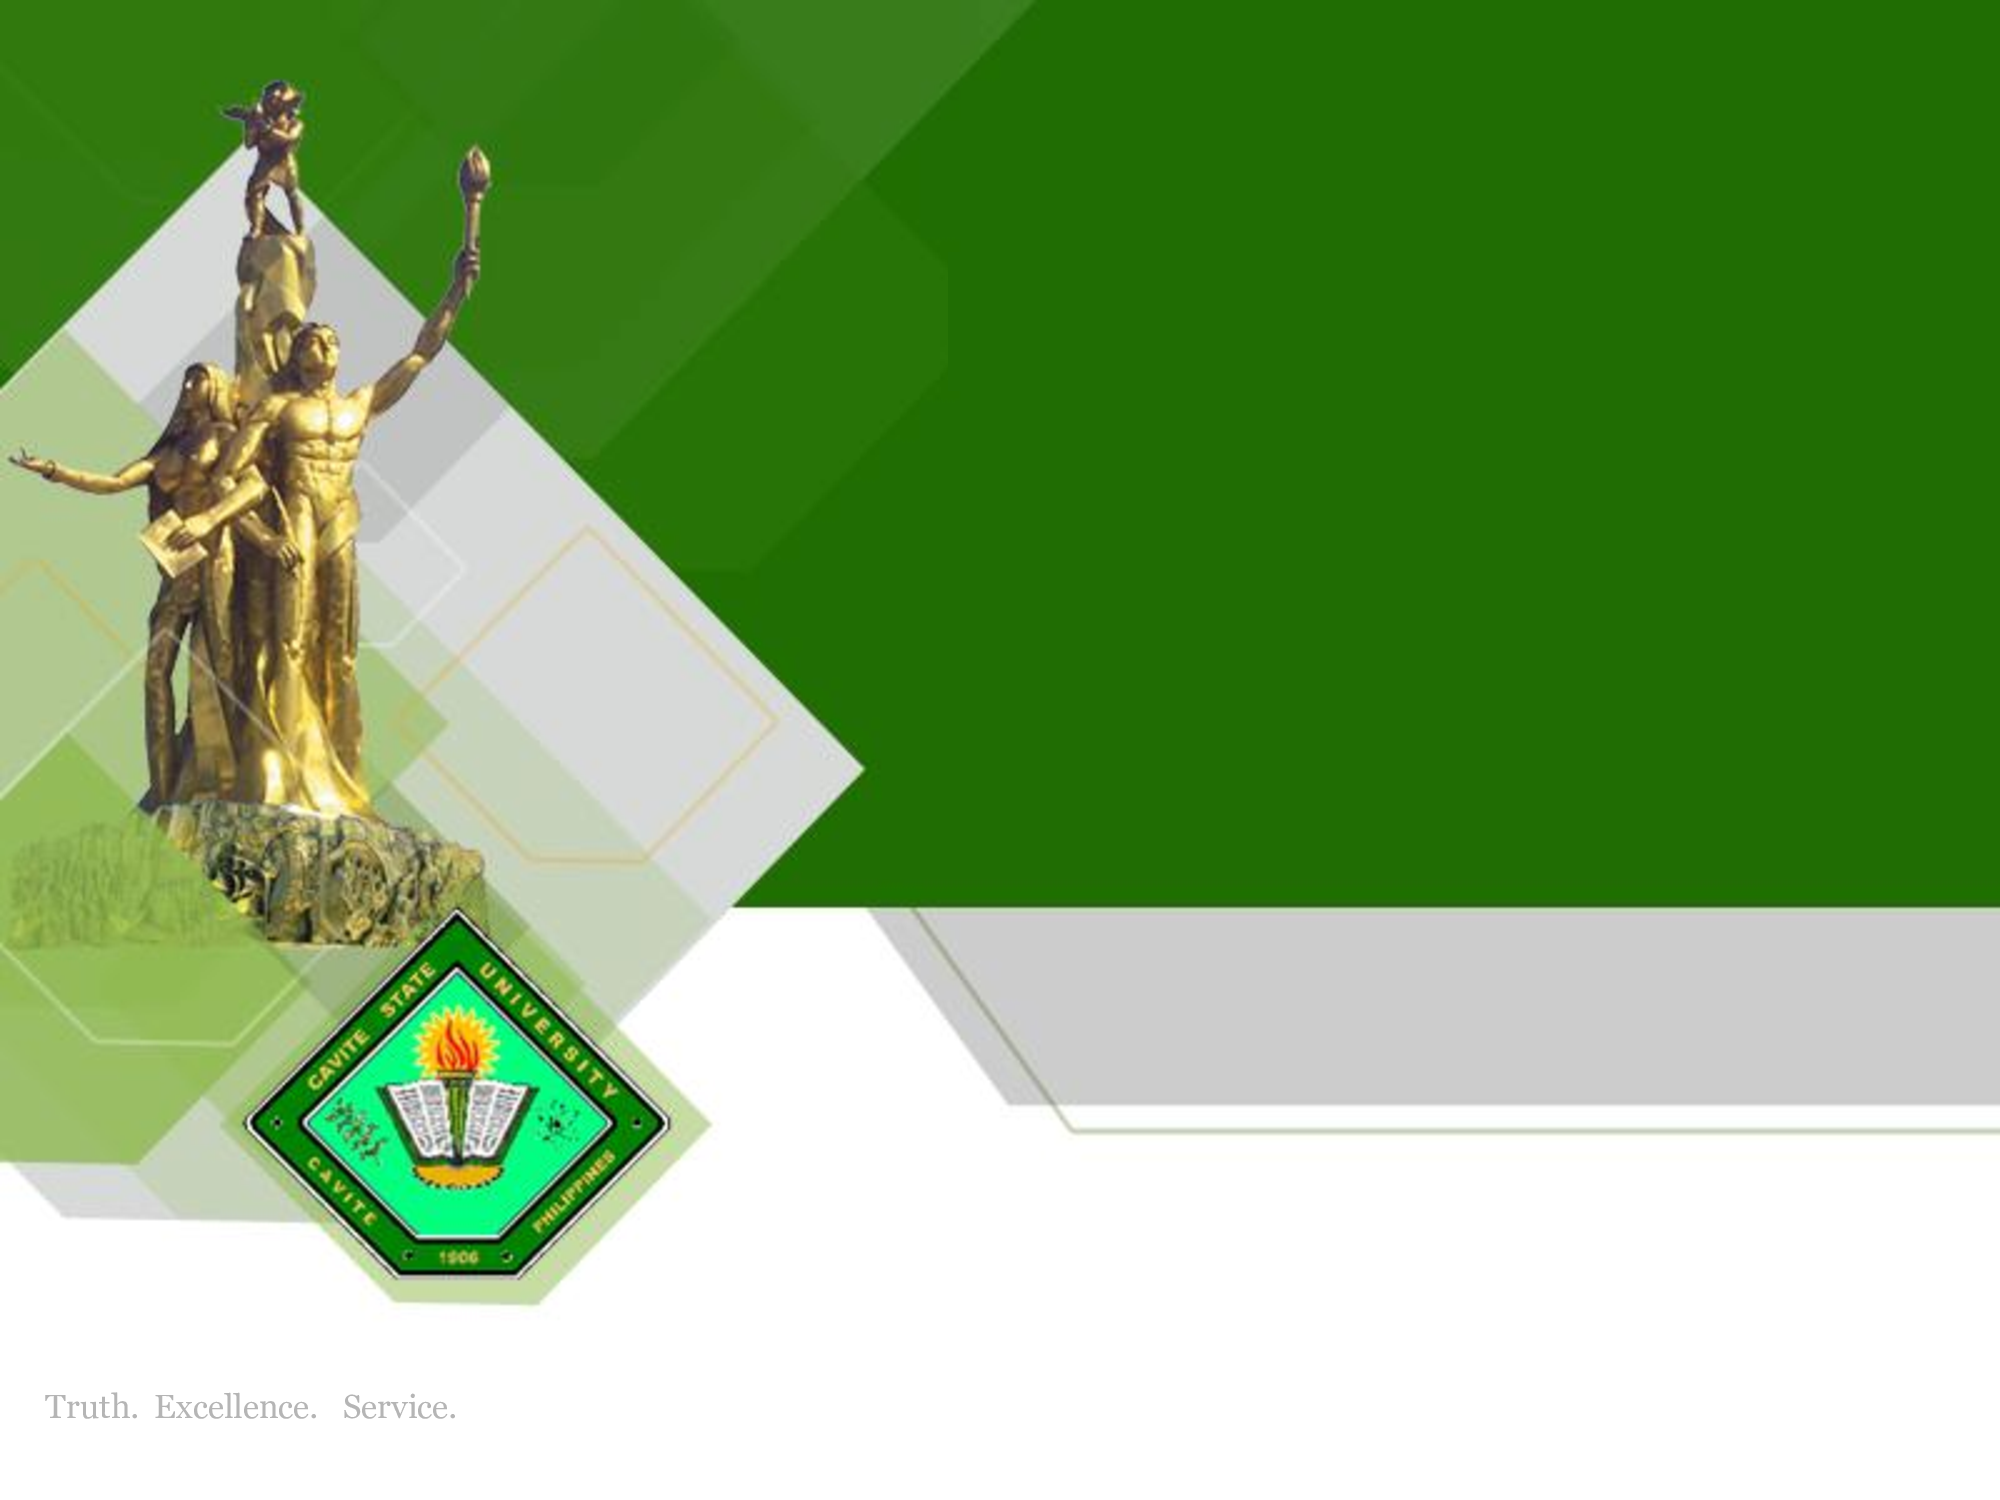
\includegraphics[width=\paperwidth,height=\paperheight,keepaspectratio]{template_title.png}}

\begin{frame}
	\begin{textblock}{6}(3.5,1.5)
		\titlepage
	\end{textblock}
\end{frame}

\setbeamertemplate{background}
{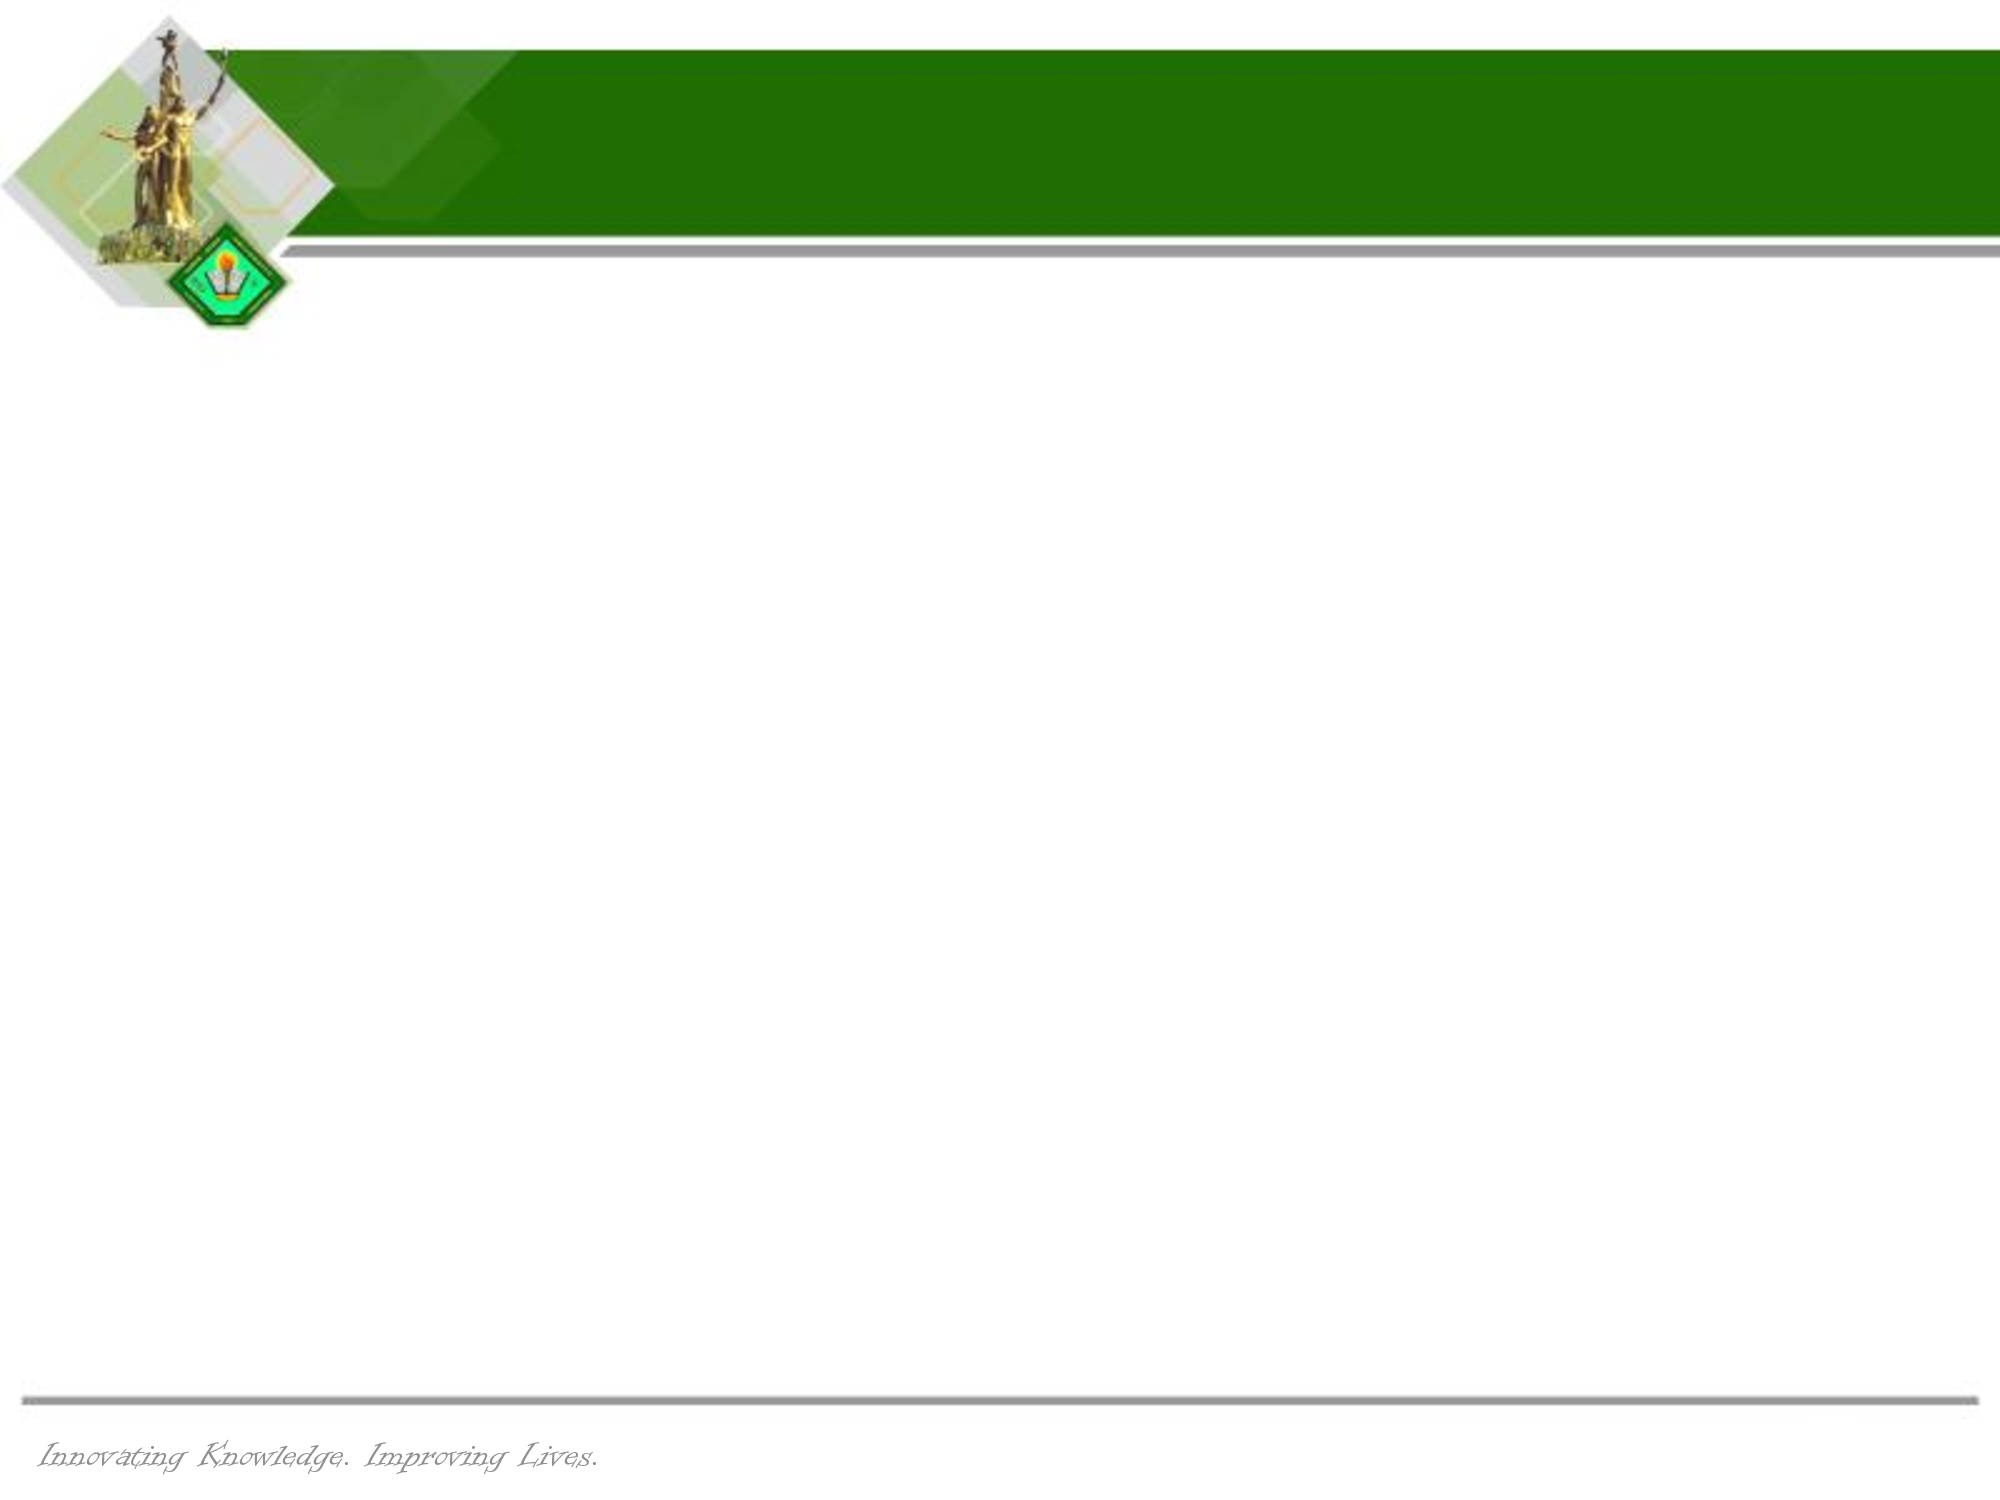
\includegraphics[width=\paperwidth,height=\paperheight,keepaspectratio]{template.png}}

\begin{frame}
	\frametitle{Introduction}
	\begin{itemize}
			\item<1-> Technology is constantly progressing and improving
			\item<2-> Programming is essential in the field of technology
			\item<3-> Programming is a discipline
			\item<4-> Programming is difficult
			\item<5-> Learning programming is more difficult
	\end{itemize}
\end{frame}

\begin{frame}<all:0>
	\frametitle{Introduction}
	\justifying
	\parx
	According to Tsai, Yang, and Chang, one of the requirements for a programmer
	is to have expertise in technical skills that include multiple programming
	languages.
\end{frame}

\begin{frame}<all:0>
	\frametitle{Introduction}
	\justifying
	\parx
	Learning programming has indeed became easier and better through the use and
	aid of technology itself. Education integrates modern tools to increase the
	rate of knowledge acquisition and absorption (Raja and Nagasubramani, 2018).
\end{frame}

\begin{frame}<all:0>
	\frametitle{Introduction}
	\justifying
	\parx
	Commonly used software for programming have numerous features that are useful
	and engaging but for learning, the features become bloat and can result in
	user fatigue (Thompson, Hamilton, and Rust, 2005).
\end{frame}

\begin{frame}
	\frametitle{Statement of the Problem}
	\justifying
	\parx
	The fundamental concepts of programming are essential basics that are necessary
	for programmers to master. Concepts such as:

	\begin{itemize}
			\item<1-> Syntax and Semantics
			\item<2-> Data Types and Data Structures
			\item<3-> Logic and Conditionals
			\item<4-> Loops and Algorithm
			\item<5-> Memory
	\end{itemize}

	\onslide<6->{are key to easily understanding and getting better at
	programming as programming is a discipline (Prahofer, Hurnaus, Wirth, and
	Mossenbock, 2007).}
\end{frame}

\begin{frame}<all:0>
	\frametitle{Statement of the Problem}
	\justifying
	\parx
	Programming is a skill which can be boring, intimidating, and unrelated to
	daily activities and experience. Programming education requires the
	assistance of technology itself through software in improving the quality of
	learning. The traditional method of pure lecture is nowadays complimented
	with the application of softwares. But most tools are not beginner-friendly
	and are cluttered with features that present confusion and steep learning
	curve in familiarity and mastery that diminish the learning experience
	(Tsukamoto et al., 2016).
\end{frame}

\begin{frame}<all:0>
	\frametitle{Statement of the Problem}
	\begin{figure}
		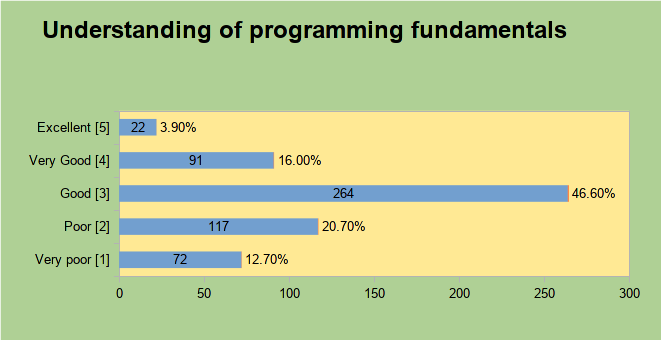
\includegraphics[scale=0.25]{results/12.png}
	\end{figure}

	\justifying
	\parx
	The assessment of the respondents under the courses with programming subjects
	shows that students are not familiar and not well versed on fundamental
	concepts and find it difficult to understand.
\end{frame}

\begin{frame}<all:0>
	\frametitle{Statement of the Problem}
	\begin{figure}
		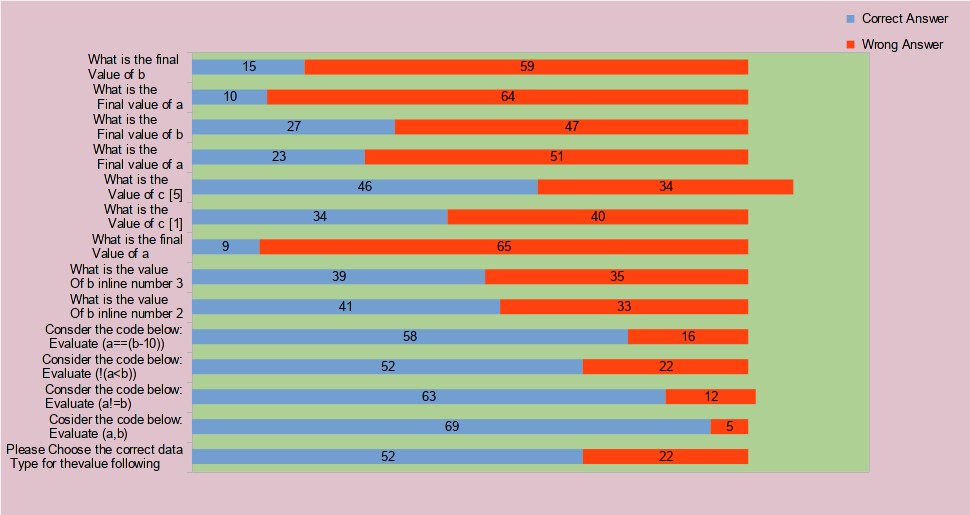
\includegraphics[scale=0.25]{results/13.png}
	\end{figure}

	\justifying
	\parx
	Basic concepts such as loops, memory management, and functions are easily
	understood individually, but combining them into a program has confused
	students. Respondents failed to correctly answer the assessment.
\end{frame}

\begin{frame}<all:0>
	\frametitle{Statement of the Problem}
	\begin{figure}
		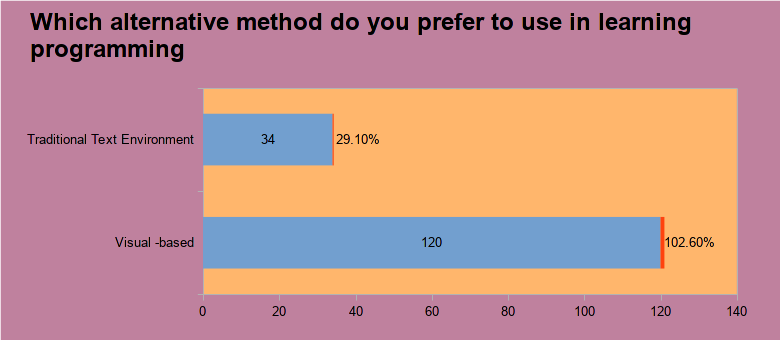
\includegraphics[scale=0.25]{results/10.png}
	\end{figure}

	\justifying
	\parx
	Survey shows that 76\% of students use outdated text-based editors in their
	laboratory classes such as Notepad++, DevC++, and TurboC/C++ , while only
	24\% use professional and modern editors for programming. This traditional
	textbased editors are general tools and are not oriented for learning of
	beginners and thus not effective.
\end{frame}

\begin{frame}<all:0>
	\frametitle{Ishikawa Diagrams}
	\begin{figure}
		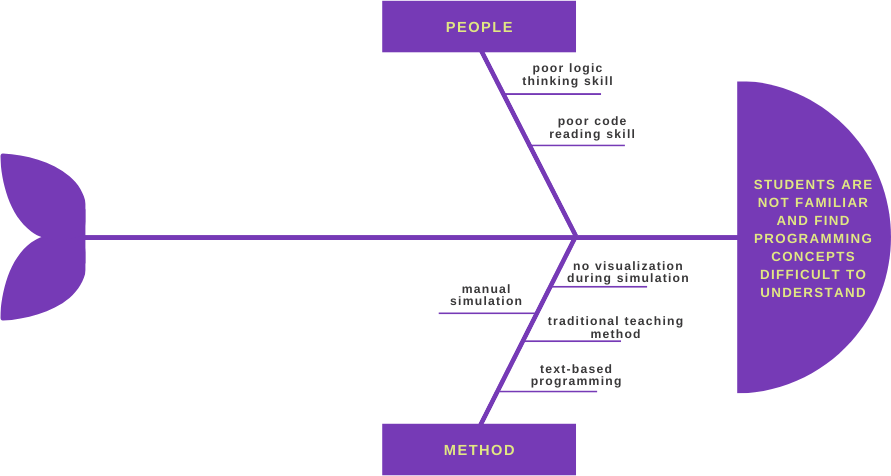
\includegraphics[width=0.8\textwidth]{figures/fishbone1.png}
	\end{figure}
	\centering
	Ishikawa diagram of students not familiar and finding programming concepts
	difficult to understand
\end{frame}

\begin{frame}<all:0>
	\frametitle{Ishikawa Diagrams}
	\begin{figure}
		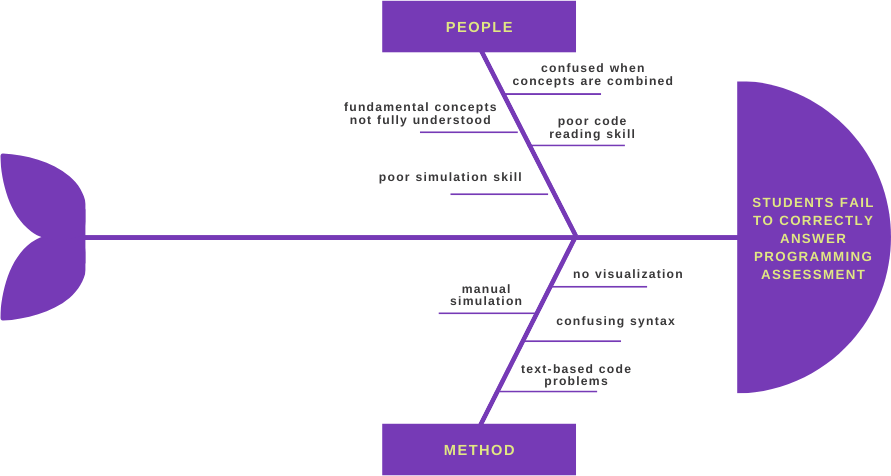
\includegraphics[width=0.8\textwidth]{figures/fishbone2.png}
	\end{figure}
	\centering
	Ishikawa diagram of students failing to correctly answer programming
	assessment
\end{frame}

\begin{frame}<all:0>
	\frametitle{Ishikawa Diagrams}
	\begin{figure}
		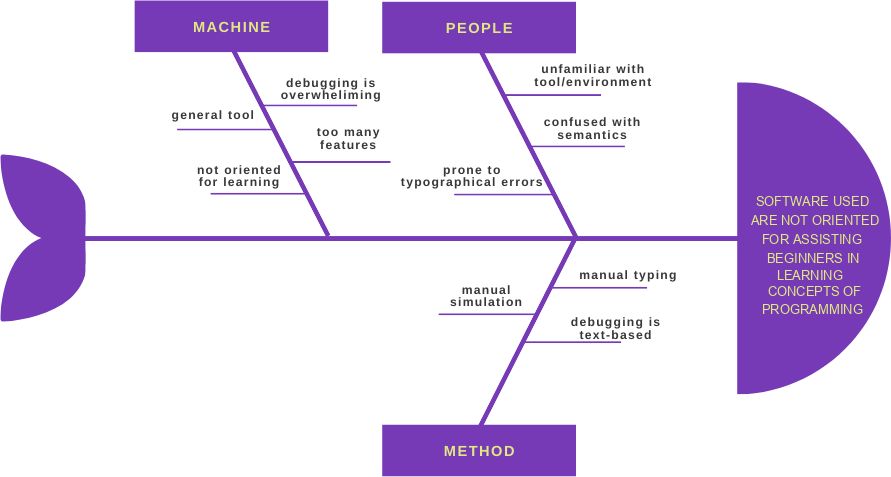
\includegraphics[width=0.8\textwidth]{figures/fishbone3.png}
	\end{figure}
	\centering
	Ishikawa diagram of the tools for programming not effective for learning
\end{frame}

\begin{frame}
	\frametitle{Objectives of the Study}
	\justifying
	\parx
	The general objective of the study is to develop a CodeNect: Visual Programming
	Software that will help in learning the fundamentals of programming.

	\parx
	Specifically, this study seeks:

	\begin{itemize}
		\item<1-> Identify the concepts learners find difficult to understand through conducted survey.
		\item<2-> Analyze the problems through a Ishikawa/Fishbone Diagram.
		\item<3-> Design the system using the Use Case Diagrams.
		\item<4-> Test the usability, functionality of the software using Experience-based test design.
		\item<5-> Evaluate the acceptability of the software using the ISO 9126.
	\end{itemize}
\end{frame}

\begin{frame}
	\frametitle{Objectives of the Study}
	\justifying
	\parx
	\begin{itemize}
		\item<1-> Develop the software with the following main features:
		\begin{columns}
			\begin{column}{.5\linewidth}
				\begin{itemize}
						\item<2-> Visual Nodes Module
						\item<3-> Filesystem Module
						\item<4-> Input/Output Module
						\item<5-> Debug Module
				\end{itemize}
			\end{column}
			\begin{column}{.5\linewidth}
				\begin{itemize}
						\item<9-> Simulation Module
						\item<7-> Transpiler Module
						\item<8-> Assessment Module
				\end{itemize}
			\end{column}
		\end{columns}
	\end{itemize}
\end{frame}

\begin{frame}
	\frametitle{Significance of the Study}
	\begin{block}{Students}
		The software helps in the education and improvement in the knowledge,
		skills, understanding, and expertise of the students and learners about
		programming. Thus, allowing them to compete and increasing the
		opportunities for their careers.
	\end{block}

	\begin{block}{Teachers}
		The software provides assistance for teachers and instructors to teach and
		demo programming concepts through visualization. This aids in relieving workload,
		stress, and maximizing lessons each class time.
	\end{block}
\end{frame}

\begin{frame}
	\frametitle{Significance of the Study}
	\begin{block}{Educational Institutions}
		The software benefits educational institutions like university for computer
		laboratory classes by providing a free software oriented for the purpose of
		learning
	\end{block}

	\begin{block}{Developers}
		The software provides learning experience for the developers and researchers
		in preparation for software development career.
	\end{block}

	\begin{block}{Researchers}
		This study serves as a guide and reference in the field of software
		development and education for future researchers.
	\end{block}
\end{frame}

\begin{frame}
	\frametitle{Conceptual Framework of the Study}
	\begin{figure}
		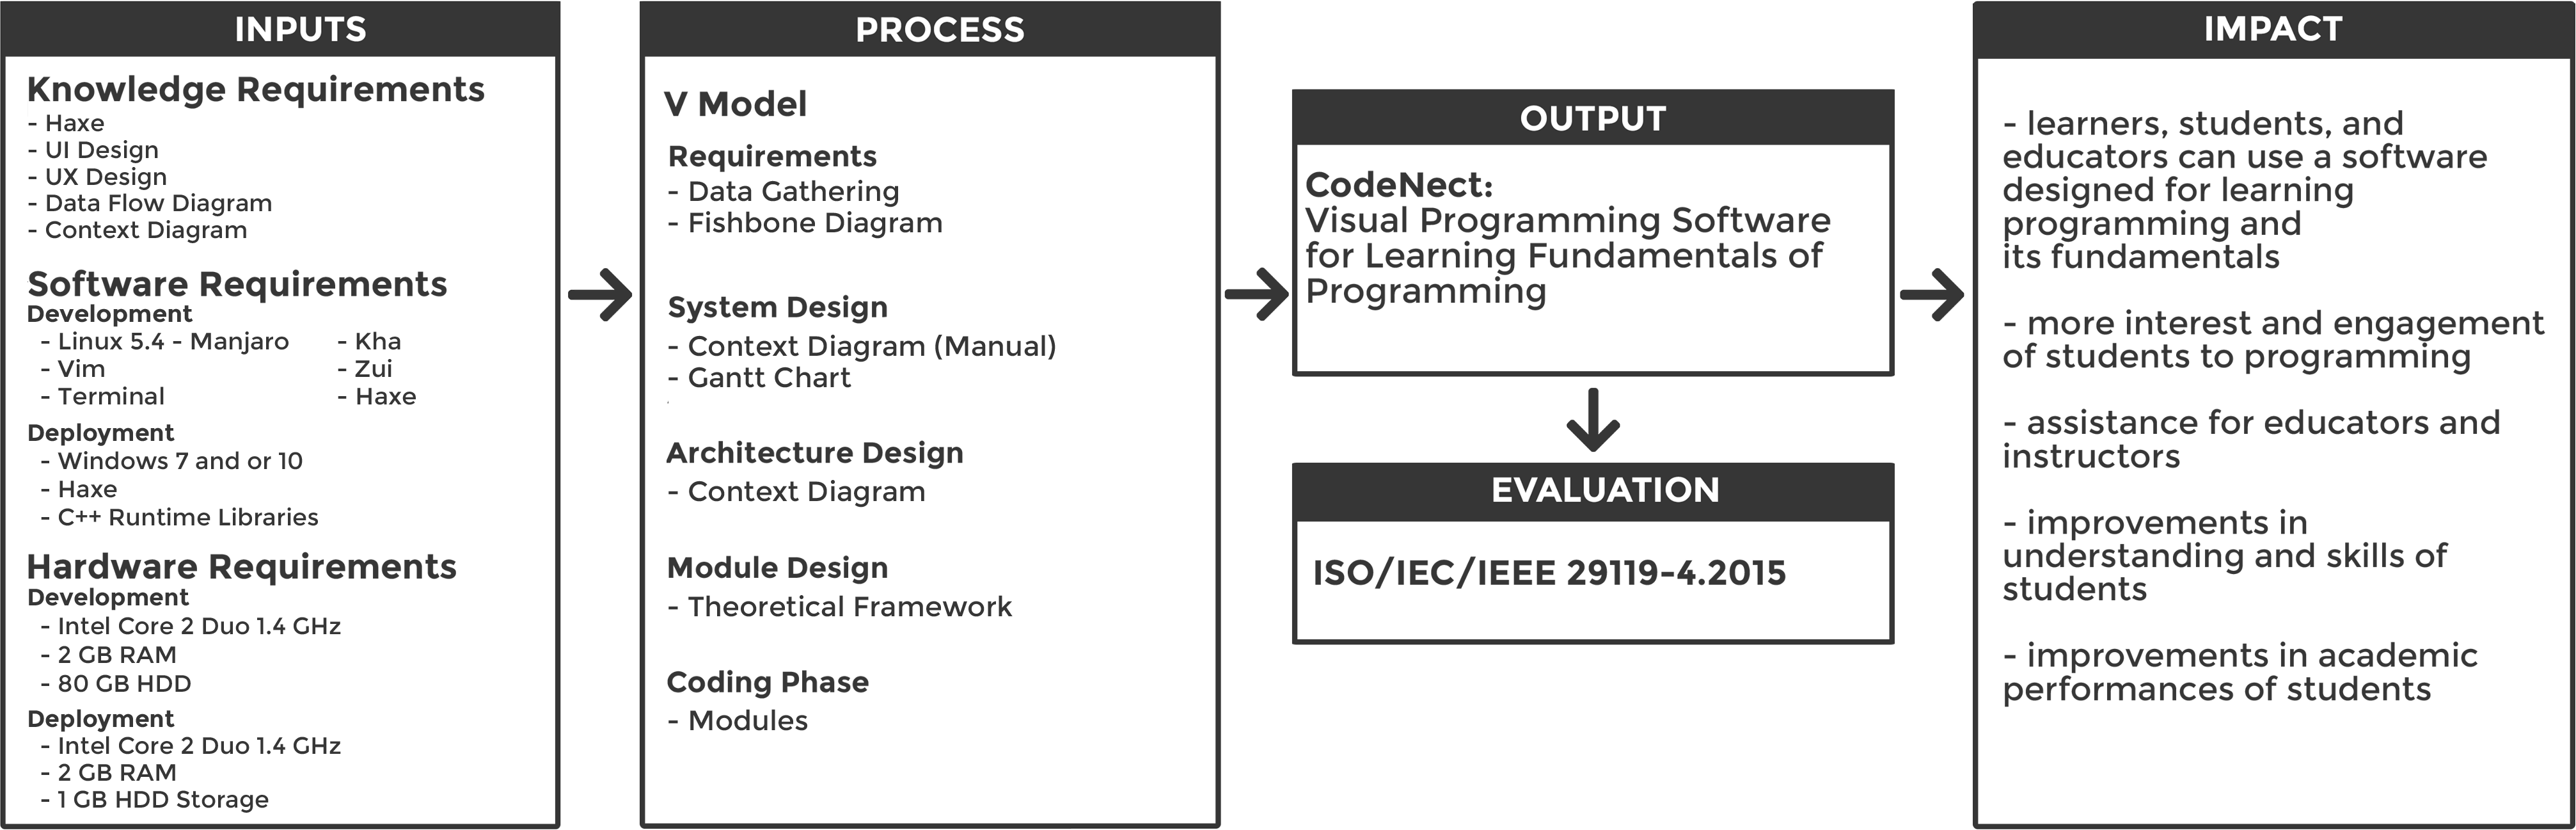
\includegraphics[width=1\textwidth]{figures/conceptual_framework.png}
	\end{figure}
\end{frame}

\begin{frame}
	\frametitle{Scope and Limitations of the Study}
	\begin{block}{Simplicity and Functionality}
		The software will prioritize simple and basic functionalities over numerous
		features for the purpose of learning and education.
	\end{block}
	\begin{block}{Stand-alone Program}
		The software will have no account management and can be run without any
		hassle. The software works perfectly in offline mode.
	\end{block}
	\begin{block}{Terminal-based}
		The software is limited to simulating text-based or command/terminal
		prompts as the priority is learning the fundamentals of programming.
	\end{block}
\end{frame}

\begin{frame}
	\frametitle{Scope and Limitations of the Study}
	\begin{block}{Visual Nodes Module}
		Nodes are graphical elements that serve as the building blocks of the
		software.  Nodes can be used as a variable, logic, and conditionals
	\end{block}
	\begin{block}{Filesystem Module}
		Serves as the interface between the software and the user’s machine for
		handling files such as creation, modification, reading, and deletion.
	\end{block}
\end{frame}

\begin{frame}
	\frametitle{Scope and Limitations of the Study}
	\begin{block}{Input/Output Module}
		The module is responsible for processing and responding events
		and performing actions based on the event such as key press, mouse click,
		and mouse movement.
	\end{block}
	\begin{block}{Debug Module}
		This module will linter and give feedback and indication to the user
		whenever there is an attempt to perform an action that is faulty in logic
	\end{block}
\end{frame}

\begin{frame}
	\frametitle{Scope and Limitations of the Study}
	\begin{block}{Simulation Module}
		The process of simulation involves the compiling, building, and running the
		visual code is executed by this module
	\end{block}
	\begin{block}{Transpiler Module}
		This module transpiles the visual code made by the user into source code in
		target programming language
	\end{block}
\end{frame}

\begin{frame}
	\frametitle{Scope and Limitations of the Study}
	\begin{block}{Assessment Module}
		The functionality of providing exercises designed for the learning of
		topics and concepts in programming and evaluation of the results are
		handled by this module
	\end{block}
\end{frame}

\begin{frame}<all:0>
	\frametitle{Related Studies}
	\begin{itemize}
		\item<1-> Prototype of Visual Programming Environment for C Language Novice Programmer (Abe, K., Fukawa, Y., \& Tanaka, T., 2019)
		\item<2-> On the Design of a Generic Visual Programming Environment (Zhang, D.-Q., \& Zhang, K.)
		\item<3-> Environment pi J for Visual Programming in Java (Prokhorov, V., \& Kosarev, V., 1999)
		\item<4-> HASKEU: An editor to support visual and textual programming in tandem (Alam, A., \& Bush, V. , 2016)
		\item<5-> The Scratch Programming Language and Environment (Maloney, J., Resnick, M., Rusk, N., Silverman, B., \& Eastmond, E. ,2010)
	\end{itemize}
\end{frame}

\begin{frame}
	\frametitle{Methodology - Materials}
	\begin{block}{Sofware Requirements - Development}
		\begin{itemize}
			\item<1-> Linux 5.4 kernel with Manjaro distribution as Operating System
			\item<2-> Terminal for running commands
			\item<3-> Vim for text and code editing
			\item<4-> GLFW and OpenGL for rendering
			\item<5-> DearImGui and ImNodes for user-interface base framework
			\item<6-> C++ programming language
		\end{itemize}
	\end{block}
\end{frame}

\begin{frame}<all:0>
	\frametitle{Methodology - Materials}
	\begin{block}{Hardware Requirements - Development}
		\begin{itemize}
			\item<1-> Laptop
			\item<2-> 2GB RAM (Random Access Memory)
			\item<3-> Intel Core 2 Duo at 1.4 GHz processor
			\item<4-> 80 GB HDD
		\end{itemize}
	\end{block}
\end{frame}

\begin{frame}<all:0>
	\frametitle{Methodology - Materials}
	\begin{block}{Sofware Requirements - Deployment}
		\begin{itemize}
			\item<1-> Microsoft Windows 7 or above
			\item<2-> C++ Runtime libraries
		\end{itemize}
	\end{block}
\end{frame}

\begin{frame}<all:0>
	\frametitle{Methodology - Materials}
	\begin{block}{Hardware Requirements - Deployment}
		\begin{itemize}
			\item<1-> Laptop or Desktop
			\item<2-> 2GB RAM (Random Access Memory)
			\item<3-> Atleast Intel Core 2 Duo at 1.4 GHz processor
			\item<4-> Atleast 1 GB HDD
		\end{itemize}
	\end{block}
\end{frame}

\begin{frame}
	\frametitle{Methodology - Method}

	\begin{block}{V-Model}
		This model follows the relationships between each of the different phases
		in the life cycle of the development process, each with an associated
		testing phase.

		The primary focus and purpose of this model is to improve the efficiency of
		development and to ensure the effectiveness of the software.
	\end{block}
\end{frame}

\begin{frame}
	\frametitle{Methodology - V-Model}
	\begin{block}{Phases of V-Model}
		\begin{itemize}
			\item<1-> Requirements
			\item<2-> System Design
			\item<3-> Architecture Design
			\item<4-> Module Design
			\item<5-> Implementation and Coding
			\item<6-> Testings
		\end{itemize}
	\end{block}
\end{frame}

\begin{frame}<all:0>
	\frametitle{Methodology - V-Model}
	\begin{block}{Requirements}
		\begin{itemize}
			\item<1-> Conduction of survey
			\item<2-> Gathering of data
			\item<3-> Conduction of assesment
		\end{itemize}

		\onslide<4->{The end results are:}
		\begin{itemize}
			\item<4-> Ishikawa Diagrams
			\item<5-> Graphical representations of data
		\end{itemize}
	\end{block}
\end{frame}

\begin{frame}<all:0>
	\frametitle{Methodology - V-Model - Requirements}
	\center{Examples of questions:}

	\begin{columns}
		\begin{column}{.5\linewidth}
			\begin{semiverbatim}
				int a = 20;

				int *b = \&a;

				(*b)++;

				1. What is the final of `b` in line 2?

				2. What is the final of `b` in line 3?
			\end{semiverbatim}
		\end{column}

		\begin{column}{.5\linewidth}
			\begin{semiverbatim}
				int a = 5;

				int b = 20;

				for (int i=a; i<b; i+=2)

				\{

						a++;

						b--;

				\}

				1. What is the final value of `a`?

				2. What is the final value of `b`?
			\end{semiverbatim}
		\end{column}
	\end{columns}
\end{frame}

\begin{frame}<all:0>
	\frametitle{Methodology - V-Model}
	\begin{block}{System Design}
		\begin{itemize}
			\item<1-> Assessment of the current manual or system
			\item<2-> Schedule of the development
		\end{itemize}

		\onslide<3->{The end results are:}
		\begin{itemize}
			\item<3-> Context Diagram (Manual)
			\item<4-> Gantt Chart
		\end{itemize}
	\end{block}
\end{frame}

\begin{frame}<all:0>
	\frametitle{Methodology - V-Model}
	\begin{block}{Architecture Design}
		\begin{itemize}
			\item<1-> Specifications as blueprint of the software
			\item<2-> Selection of libraries and tools to be used
		\end{itemize}

		\onslide<3->{The end result is:}
		\begin{itemize}
			\item<3-> Context Diagram
		\end{itemize}
	\end{block}
\end{frame}

\begin{frame}<all:0>
	\frametitle{Methodology - V-Model}
	\begin{block}{Module Design}
		\begin{itemize}
			\item<1-> Identification and definition of each module
			\item<2-> Scope and integration of the modules to the system
		\end{itemize}

		\onslide<3->{The end result is:}
		\begin{itemize}
			\item<3-> Theoretical Framework
		\end{itemize}
	\end{block}
\end{frame}

\begin{frame}<all:0>
	\frametitle{Methodology - V-Model}
	\begin{block}{Implementation and Coding}
		\begin{itemize}
			\item<1-> Start of programming and development
			\item<2-> Compilation and running of the modules
			\item<3-> Integration and coupling of the modules as a software
		\end{itemize}

		\onslide<4->{The end results are:}
		\begin{itemize}
			\item<4-> Modules
		\end{itemize}
	\end{block}
\end{frame}

\begin{frame}<all:0>
	\frametitle{Methodology - V-Model}
	\begin{block}{Testing}
		\begin{itemize}
			\item<1-> Application of tests
			\item<2-> Fixing of bugs, errors, and misbehaviors
		\end{itemize}

		\onslide<3->{To make sure of the following for the quality of the software:}
		\begin{itemize}
			\item<3-> Functionality
			\item<4-> Efficiency
			\item<5-> Usability
			\item<6-> Portability
			\item<7-> Reliability
		\end{itemize}
	\end{block}
\end{frame}

\begin{frame}<all:0>
	\frametitle{Methodology - V-Model}
	\begin{block}{Evaluation}
		The ISO 9126 Software Engineering - Product Quality is a a set of standards for
		software testing internationally recognized and approved. Its goal is to
		address well known biases of human that has an effect on the delivery and
		perception of a software project. This standard defines the following for usage
		with software development lifecycle: maintanability, efficiency, portability,
		reliability, functionality, and usability of the software product.
	\end{block}
\end{frame}

\begin{frame}<all:0>
	\frametitle{Methodology - V-Model - Evaluation}
	\begin{block}{Evaluation}
		\begin{itemize}
			\item<1-> Respondents will be tasked to solve simple coding exercises
			\item<2-> Respondents will be given a feedback form for assessment
			\item<3-> Assessment of the respondents' experience with using the software
			\item<4-> Evaluation of their solution/answer to coding exercises
			\item<5-> Comparision of the results
		\end{itemize}
	\end{block}
\end{frame}

\begin{frame}
	\frametitle{System Architecture}
	\begin{figure}
		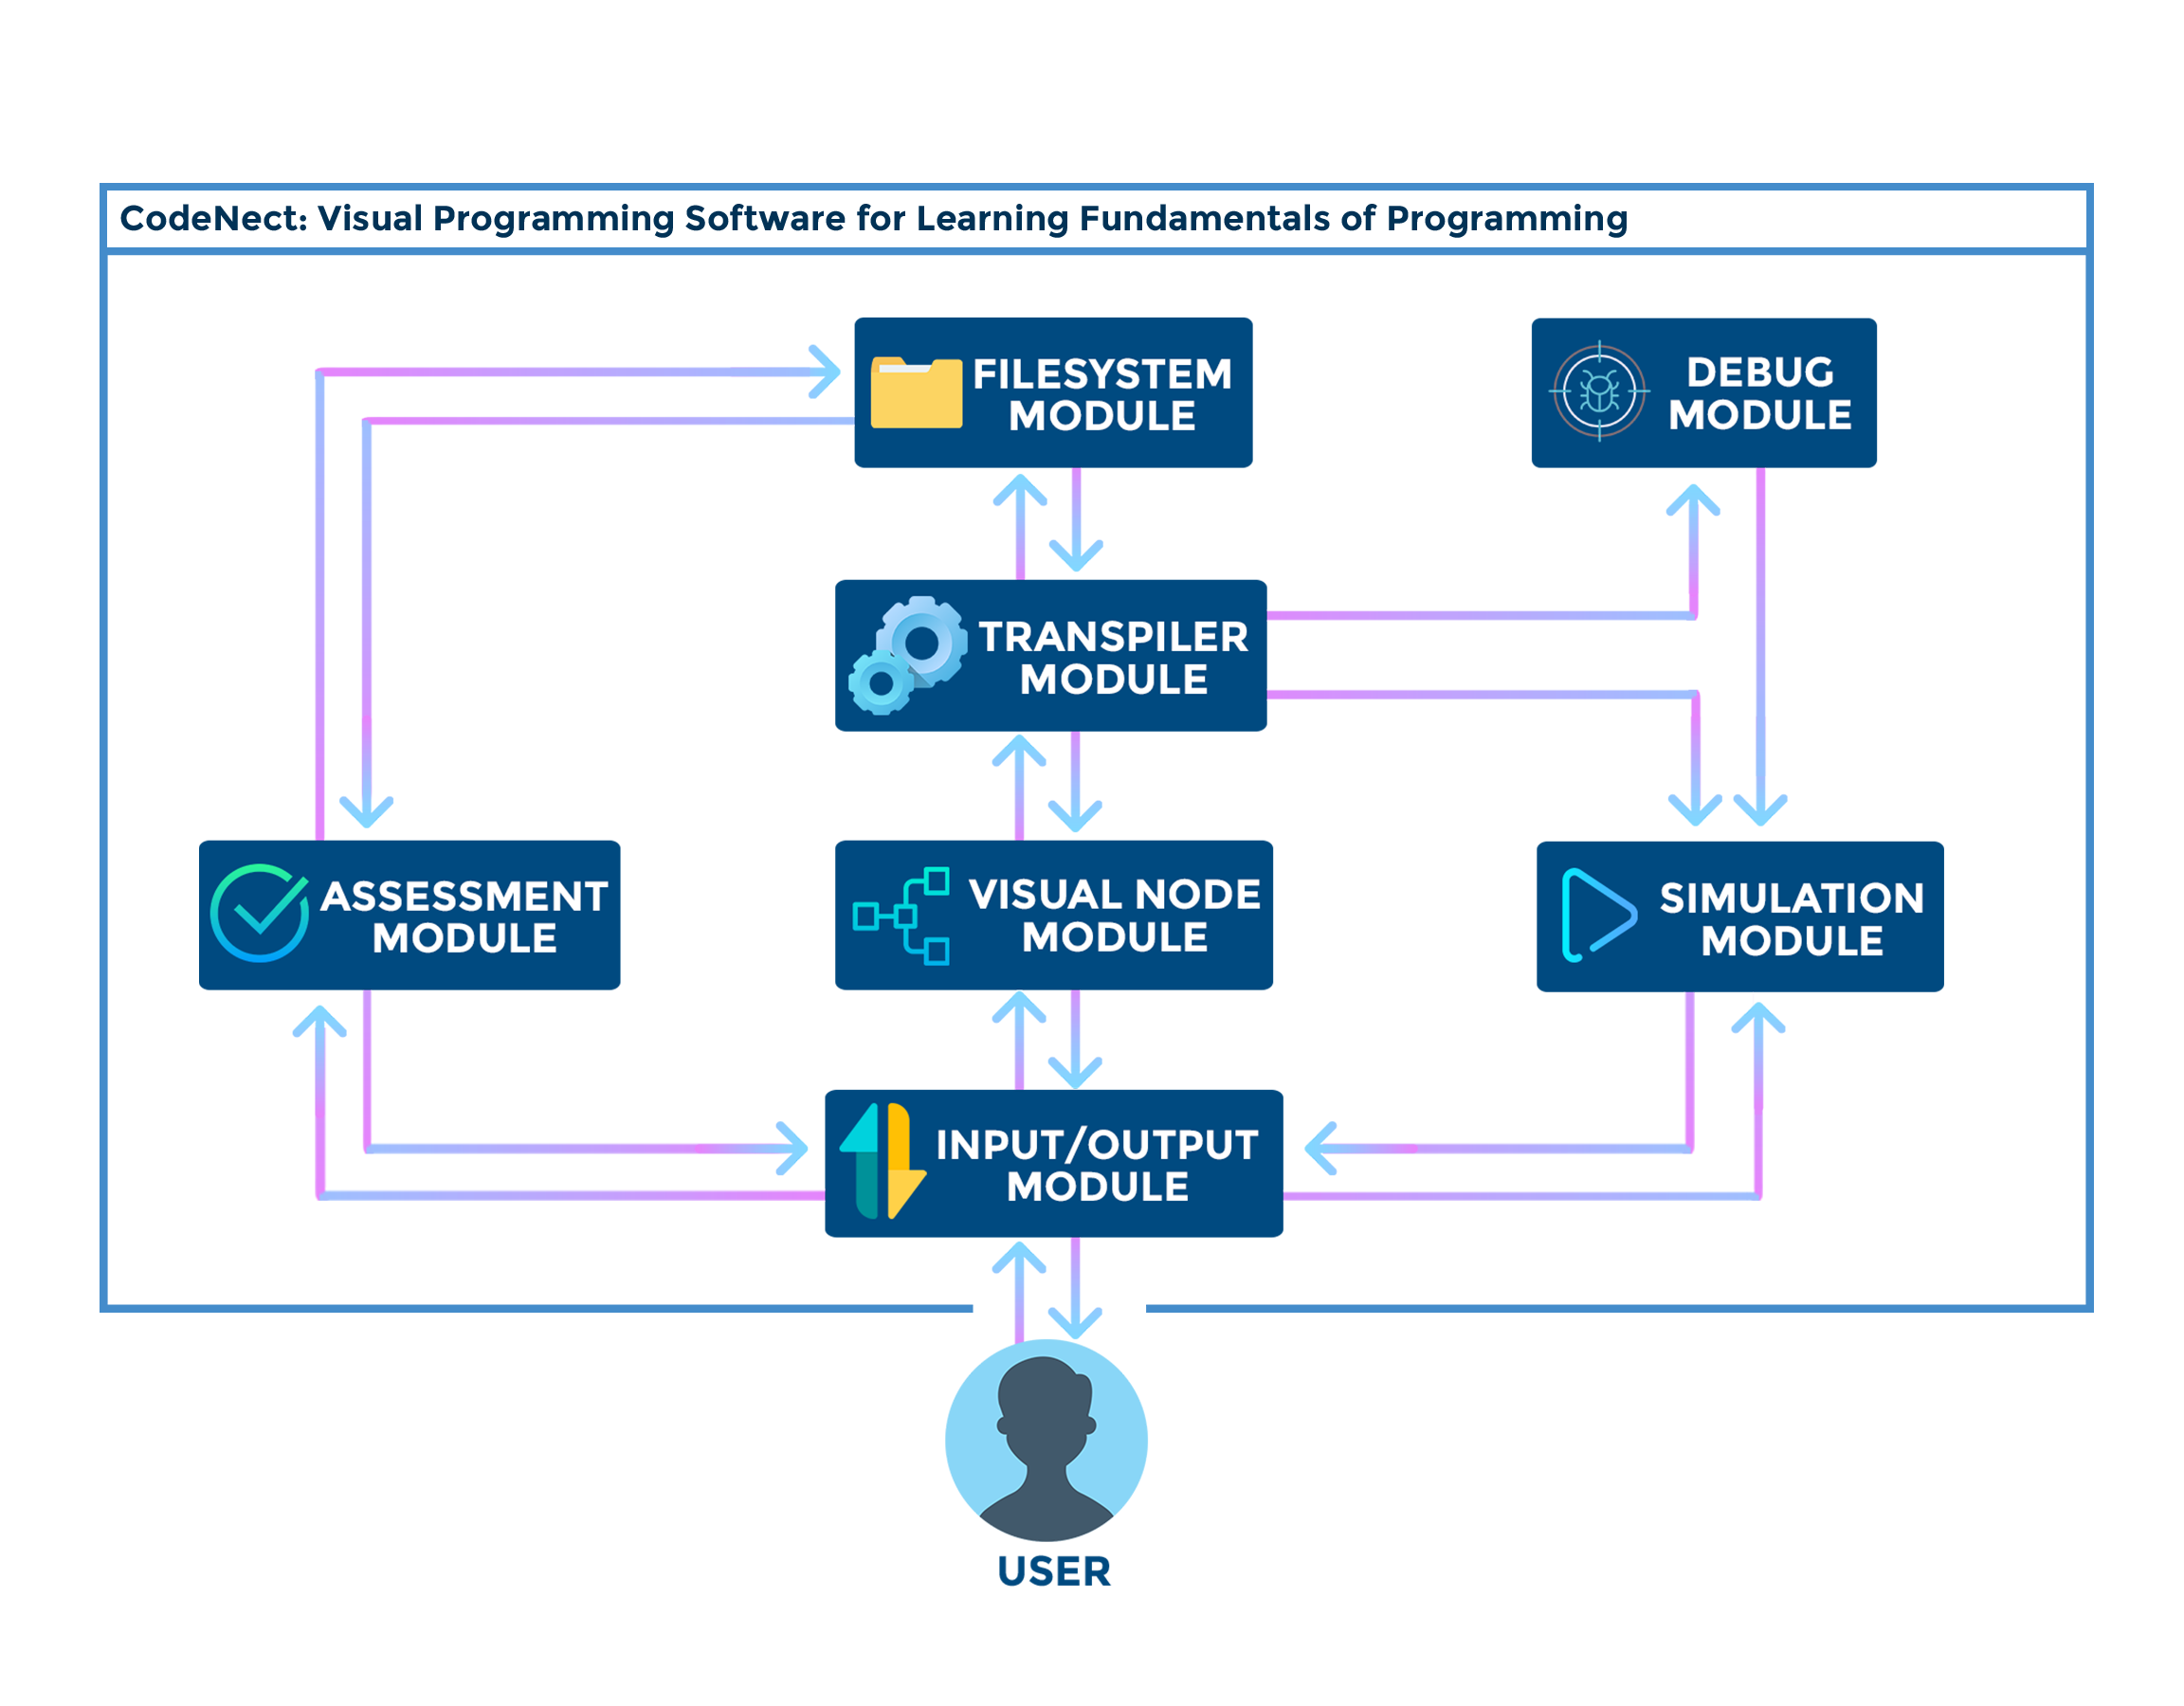
\includegraphics[width=0.8\textwidth]{figures/theoretical_framework.png}
	\end{figure}
\end{frame}

\begin{frame}
	\frametitle{Results and Discussion}
	\begin{block}{Likert Scale for Software Evaluation}
		\begin{figure}
			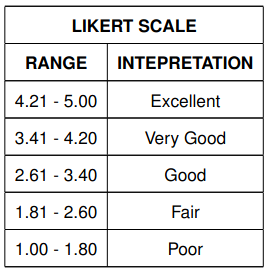
\includegraphics[width=0.5\textwidth]{figures/likert_scale.png}
		\end{figure}
	\end{block}
\end{frame}

\begin{frame}
	\frametitle{Technical Evaluation}
	\begin{block}{Technical Evaluators}
		\begin{itemize}
			\item<1-> 10 IT/CS professionals
			\item<2-> Software downloaded from Google Drive
			\item<3-> Software evaluated through Google Form
		\end{itemize}
	\end{block}
\end{frame}

\begin{frame}
	\frametitle{Technical Evaluation}
	\begin{block}{Summary Table for the Overall of the Software}
		\begin{figure}
			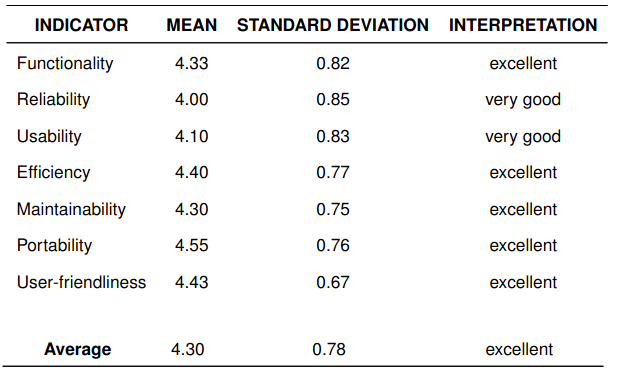
\includegraphics[width=0.8\textwidth]{figures/res_tech_overall.png}
		\end{figure}
	\end{block}
\end{frame}

\begin{frame}
	\frametitle{Technical Evaluation}
	\begin{block}{Summary Table for the Functionality of the Software}
		\begin{figure}
			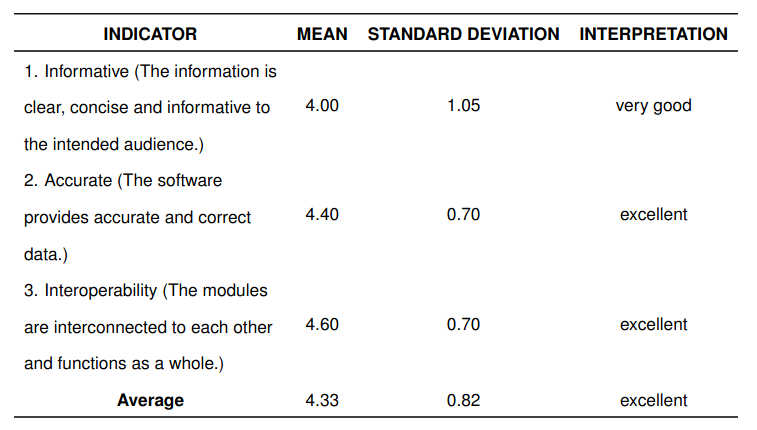
\includegraphics[width=0.8\textwidth]{figures/res_tech_functionality.png}
		\end{figure}
	\end{block}
\end{frame}

\begin{frame}
	\frametitle{Technical Evaluation}
	\begin{block}{Summary Table for the Reliability of the Software}
		\begin{figure}
			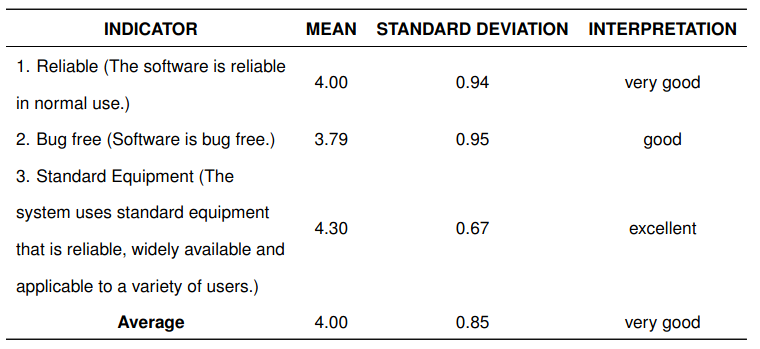
\includegraphics[width=0.8\textwidth]{figures/res_tech_reliability.png}
		\end{figure}
	\end{block}
\end{frame}

\begin{frame}
	\frametitle{Technical Evaluation}
	\begin{block}{Summary Table for the Usability of the Software}
		\begin{figure}
			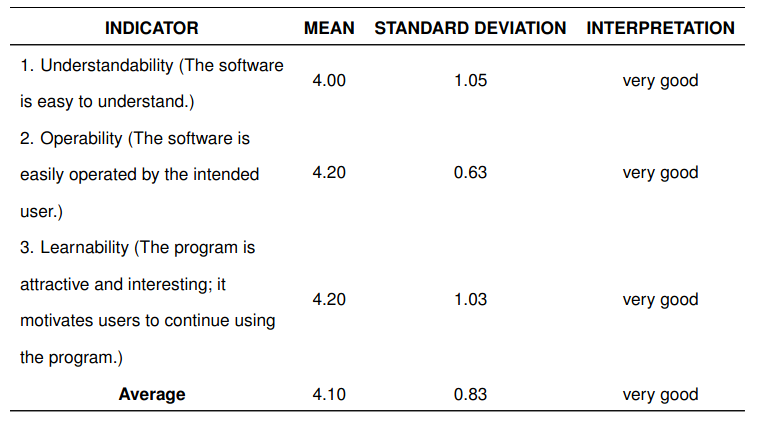
\includegraphics[width=0.8\textwidth]{figures/res_tech_usability.png}
		\end{figure}
	\end{block}
\end{frame}

\begin{frame}
	\frametitle{Technical Evaluation}
	\begin{block}{Summary Table for the Efficiency of the Software}
		\begin{figure}
			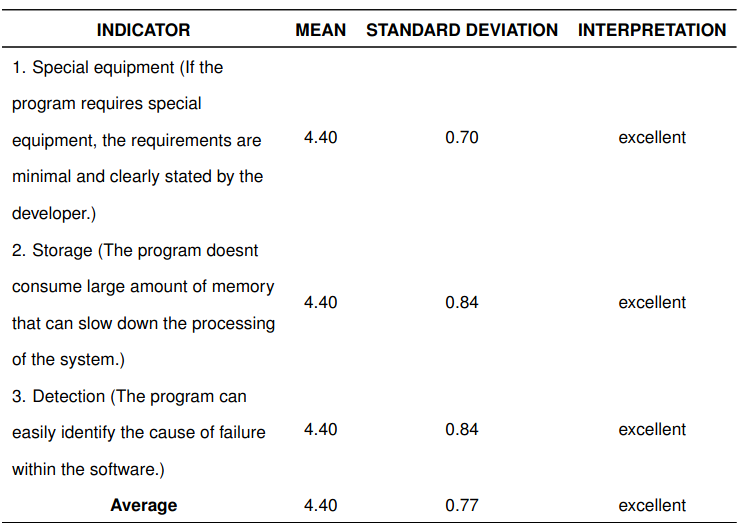
\includegraphics[width=0.8\textwidth]{figures/res_tech_efficiency.png}
		\end{figure}
	\end{block}
\end{frame}

\begin{frame}
	\frametitle{Technical Evaluation}
	\begin{block}{Summary Table for the Maintainability of the Software}
		\begin{figure}
			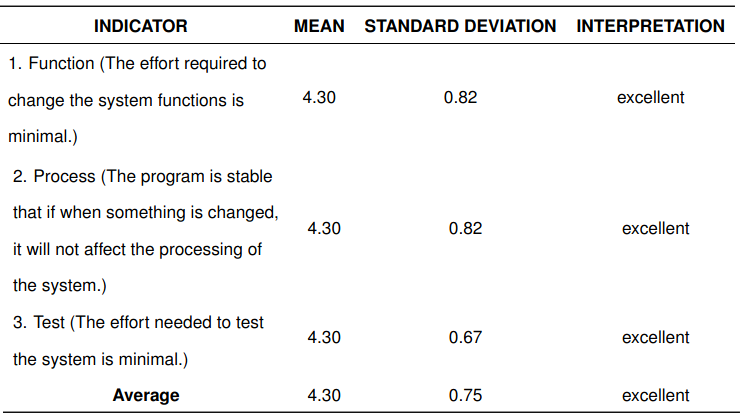
\includegraphics[width=0.8\textwidth]{figures/res_tech_maintainability.png}
		\end{figure}
	\end{block}
\end{frame}

\begin{frame}
	\frametitle{Technical Evaluation}
	\begin{block}{Summary Table for the Portability of the Software}
		\begin{figure}
			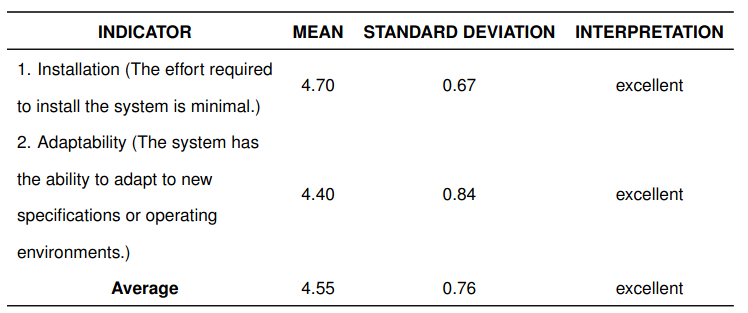
\includegraphics[width=0.8\textwidth]{figures/res_tech_portability.png}
		\end{figure}
	\end{block}
\end{frame}

\begin{frame}
	\frametitle{Technical Evaluation}
	\begin{block}{Summary Table for the User-Friendliness of the Software}
		\begin{figure}
			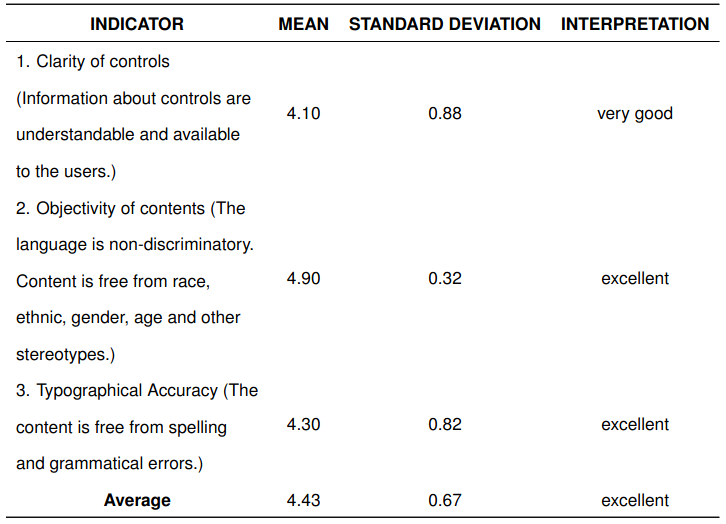
\includegraphics[width=0.8\textwidth]{figures/res_tech_uf.png}
		\end{figure}
	\end{block}
\end{frame}

\begin{frame}
	\frametitle{Technical Evaluation}
	\begin{block}{Feedbacks}
		\begin{figure}
			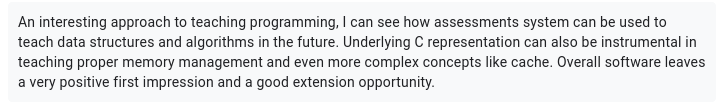
\includegraphics[width=\textwidth]{figures/feedbacks/tech1.png}
		\end{figure}
		\begin{figure}
			
\includegraphics[width=\textwidth]{figures/feedbacks/tech2.png}
		\end{figure}
		\begin{figure}
			
\includegraphics[width=\textwidth]{figures/feedbacks/tech3.png}
		\end{figure}
	\end{block}
\end{frame}

% NON-TECH
\begin{frame}
	\frametitle{Non-Technical Evaluation}
	\begin{block}{Non-Technical Evaluators}
		\begin{itemize}
			\item<1-> 12 students with programming subjects
			\item<2-> Software downloaded from Google Drive
			\item<3-> Software evaluated through Google Form
			\item<4-> YouTube video for tutorial on basic usage of the software
		\end{itemize}
	\end{block}
\end{frame}

\begin{frame}
	\frametitle{Non-Technical Evaluation}
	\begin{block}{Summary Table for the Overall of the Software}
		\begin{figure}
			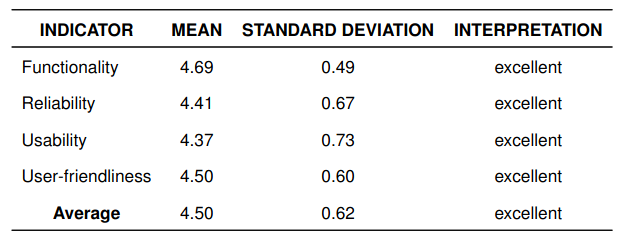
\includegraphics[width=0.8\textwidth]{figures/res_non_tech_overall.png}
		\end{figure}
	\end{block}
\end{frame}

\begin{frame}
	\frametitle{Non-Technical Evaluation}
	\begin{block}{Summary Table for the Functionality of the Software}
		\begin{figure}
			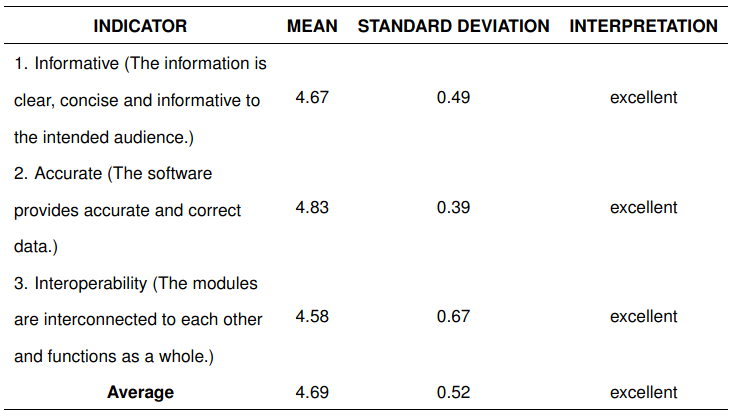
\includegraphics[width=0.8\textwidth]{figures/res_non_tech_functionality.png}
		\end{figure}
	\end{block}
\end{frame}

\begin{frame}
	\frametitle{Non-Technical Evaluation}
	\begin{block}{Summary Table for the Reliability of the Software}
		\begin{figure}
			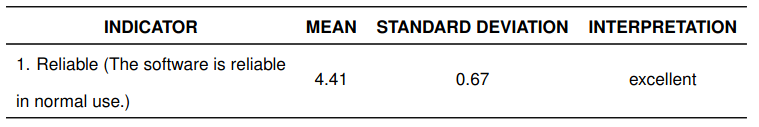
\includegraphics[width=0.8\textwidth]{figures/res_non_tech_reliability.png}
		\end{figure}
	\end{block}
\end{frame}

\begin{frame}
	\frametitle{Non-Technical Evaluation}
	\begin{block}{Summary Table for the Usability of the Software}
		\begin{figure}
			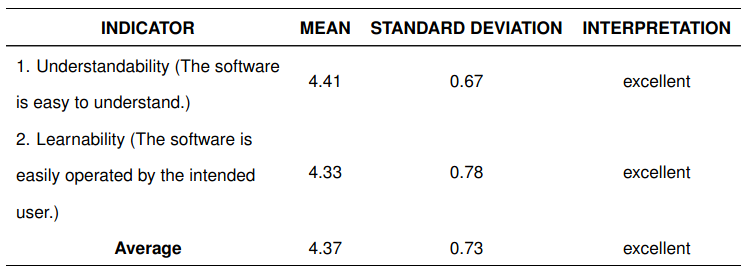
\includegraphics[width=0.8\textwidth]{figures/res_non_tech_usability.png}
		\end{figure}
	\end{block}
\end{frame}

\begin{frame}
	\frametitle{Non-Technical Evaluation}
	\begin{block}{Summary Table for the User-Friendliness of the Software}
		\begin{figure}
			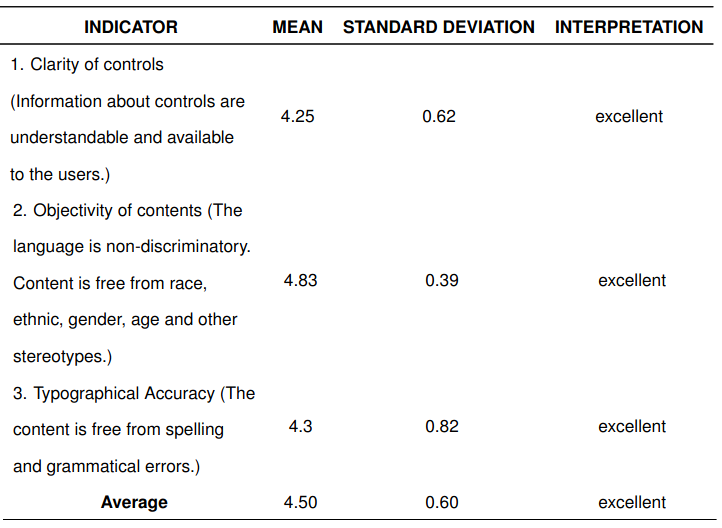
\includegraphics[width=0.8\textwidth]{figures/res_non_tech_uf.png}
		\end{figure}
	\end{block}
\end{frame}

\begin{frame}
	\frametitle{Non-Technical Evaluation}
	\begin{block}{Feedbacks}
		\begin{figure}
			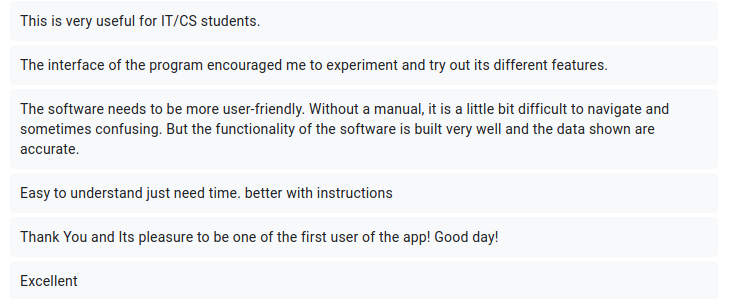
\includegraphics[width=\textwidth]{figures/feedbacks/nontech1.png}
		\end{figure}
		\begin{figure}
			
\includegraphics[width=\textwidth]{figures/feedbacks/nontech2.png}
		\end{figure}
	\end{block}
\end{frame}

\begin{frame}
	\frametitle{Summary}
	\begin{itemize}
		\item<1-> Visual Programming Software for Learning Fundamentals of Programming
		\item<2-> Uses visual elements instead of traditional text-based programming
		\item<3-> Software usable by anyone with interest in learning programming
		\item<4-> Supplementary software for instructors of programming
	\end{itemize}
\end{frame}

\begin{frame}
	\frametitle{Summary}
	\begin{block}{Seven Modules}
		\begin{itemize}
			\item<1-> Visual Nodes Module
			\item<2-> Input/Output Module
			\item<3-> Filesystem Module
			\item<4-> Transpiler Module
			\item<5-> Debug Module
			\item<6-> Simulation Module
			\item<7-> Assessment Module
		\end{itemize}
	\end{block}
\end{frame}

\begin{frame}
	\frametitle{Summary}
	\begin{block}{Evaluation}
		\begin{itemize}
			\item<1-> 10 Technical Evaluators
			\item<2-> 12 Non-Technical Evaluators
			\item<3-> ISO 9126
			\item<4-> Overall software evaluated as "EXCELLENT"
		\end{itemize}
	\end{block}
\end{frame}

\begin{frame}
	\frametitle{Conclusion}
	\begin{itemize}
		\item<1-> Seven modules developed and completed
		\item<2-> Unit test and Integration test
		\item<3-> Technical evaluation overall mean = 4.30 (EXCELLENT)
		\item<4-> Technical evaluation overall mean = 4.50 (EXCELLENT)
	\end{itemize}
\end{frame}

\begin{frame}
	\frametitle{Conclusion}
	\justifying
	\parx
	The lack of familiarity when it comes to visual programming has affected the
	metrics for usability for both the non-technical and technical evaluators
	as compared to traditional text-based programming, visual programming is
	rarely used or known.
\end{frame}

\begin{frame}
	\frametitle{Unit Test}
	\begin{figure}
		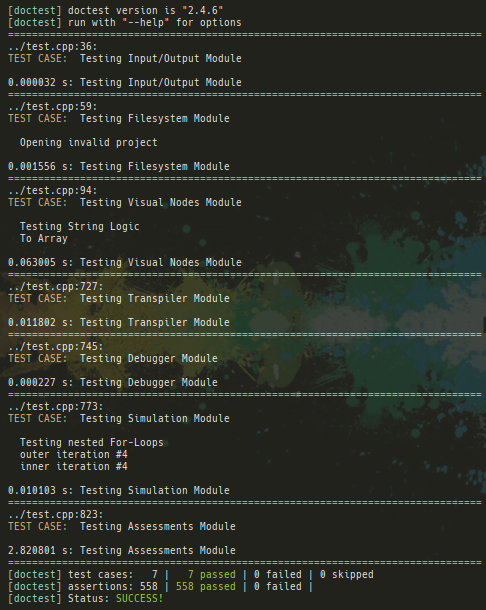
\includegraphics[width=0.5\textwidth]{figures/unit_test.png}
	\end{figure}
\end{frame}

\begin{frame}
	\frametitle{Recommendation}
	\begin{itemize}
		\item<1-> Add more programming language target for transpilation. e.g Java
		\item<2-> Increase the number of available nodes that can be used
		\item<3-> Expand the number of assessment exercises
		\item<4-> Expand the number of documents for guidelines and solutions
		\item<5-> In-depth tutorial/demo for absolute beginners
	\end{itemize}
\end{frame}

% \ui{final1}
% \ui{final2}
% \ui{final3}
% \ui{final4}
% \ui{final5}
% \ui{final6}

\begin{frame}
	\centering
	\huge Thank you so much and God bless all!
\end{frame}

\end{document}
